\section{Experimentación}
\label{sec:experimentacion}

Pasamos a experimentar sobre distintos parámetros.
Para evitar realizar \textit{overfitting} sobre una tomografía particular,
intentaremos realizar los experimentos sobre las
3 imágenes tomográficas provistas por la cátedra,
modificadas para que sean cuadradas.

\begin{figure}[H]
	\centering
    \begin{subfigure}[t]{0.3\textwidth}
        \centering
        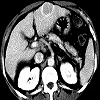
\includegraphics[height=1.0in]{../data/tomo.png}
        \caption{Tomografía 1 \footnote{Archivo tomo.png}}
    \end{subfigure}
    ~ 
    \begin{subfigure}[t]{0.3\textwidth}
        \centering
        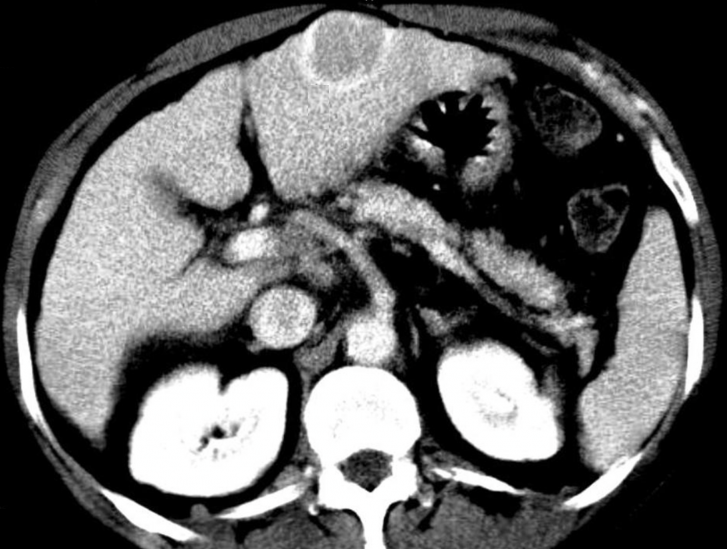
\includegraphics[height=1.0in]{../data/tomo2.png}
        \caption{Tomografía 2 \footnote{Archivo tomo2.png}}
	\label{tomo:2}
    \end{subfigure}
    ~ 
    \begin{subfigure}[t]{0.3\textwidth}
        \centering
        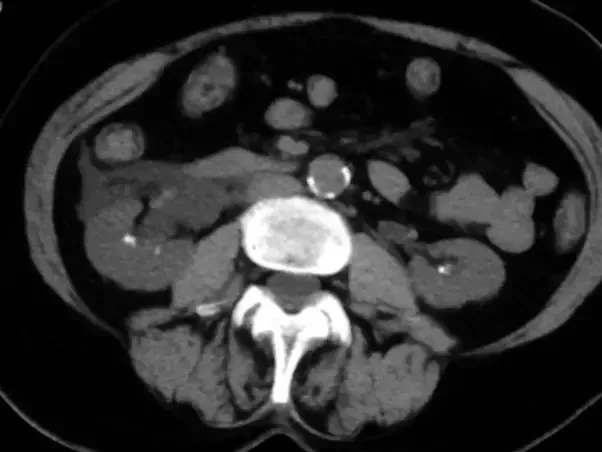
\includegraphics[height=1.0in]{../data/tomo3.png}
        \caption{Tomografía 3 \footnote{Archivo tomo3.png}}
    \end{subfigure}
    \caption{Tomografías utilizadas}
	\label{fig:tomos}
\end{figure}
% TODO: hablar de nivel de discretizacion

Proponemos 4 modelos de rayos distintos, con los cuales haremos las pruebas:

\begin{itemize}
	\item Rayos aleatorios, o \textit{random}: utilizados como base.
		Nos da una idea del comportamiento de los algoritmos.
	\item Rayos rotados, o \textit{rotated}: modelan un tomógrafo en el que el emisor de rayos
		rota alrededor del objeto, lanzando rayos que pasan por el centro del mismo. Nuestro modelo de rayos no nos va a permitir usar este método para valores de $n$ muy altos.
	\item Rayos laterales, o \textit{lateralBorders}: modela un tomógrafo en el que los rayos surgen
		desde focos a la derecha y a la izquierda de las imágenes.
	\item Rayos de todos los bordes, o \textit{allBorders}: modela un tomógrafo en el que los rayos surgen
		desde focos en los cuatro lados de la imagen.
\end{itemize}

Decidimos usar valores de \verb|n| que sean múltiplos de las imágenes originales para la experimentacion. El método de la potencia lo corrimos con 100 iteraciones como mencionamos en la sección \ref{sec:desarrollo-svd}.

% TODO: poner imagen que ilustre los rayos?
% TODO: contar que numero de iteraciones usamos en el metodo de la potencia?

\subsection{Métricas}
\label{sec:exp-metrics}

Para medir la efectividad de nuestras reconstrucciones,
se utiliza como métricas el Error Cuadrático Medio (ECM o MSE por sus siglas en inglés)
y la Proporción Máxima de Señal a Ruido (PSNR).

\begin{equation*}
   \verb|PSNR| = 10 \times \log_{10}(\verb|MAX|^2_{u}/\verb|ECM|)
\end{equation*}

donde $\verb|MAX|^2_{u}$ define el rango máximo de la imagen y \verb|ECM| es el error cuadrático medio donde se compara la imagen ideal a la imagen reconstruida.\\


Dado que utilizaremos discretizaciones de tamaño mucho menor al de las imágenes originales,
para poder compararlas con nuestras reconstrucciones,
reducimos las dimensiones de las imágenes originales utilizando \textit{GIMP}\footnote{GNU Image Manipulation Program https://www.gimp.org/}.
Estas imágenes reducidas \textbf{solamente son usadas para comparar},
nunca como \textit{input} para la simulación.

\subsection{Experimentación sobre nivel de ruido y discretización}
\label{sec:exp-noise}

Como contamos en la sección \ref{sec:desarrollo-noise},
consideramos de interés ver cómo se comporta nuestro modelo frente a distintos niveles de ruido.

Decidimos probar con ruido nulo para saber cual es la mejor métrica que se podría llegar a tener,
a pesar de que utilizando instrumentos de medición reales, este caso no existe.
Además utilizamos valores extremadamente altos de ruido para ver qué sucede en estos casos.
Nuestra hipótesis es que a medida que suba el ruido, empeoren las métricas.

En particular, a partir de cierto nivel de ruido (que esperamos cercano al 3\%),
las reconstrucciones deberían dejar de tener sentido, acercándose a un techo en el \textit{ECM}.
Para realizar estos experimentos, decidimos que la relación rayos/pixeles sea de aproximadamente 2.

% TODO: graficos? sucedio? tire fruta?
% Nombrar que algunos no pudieron conseguir todos los eigenvalues
\begin{figure}[H]
    \centering
    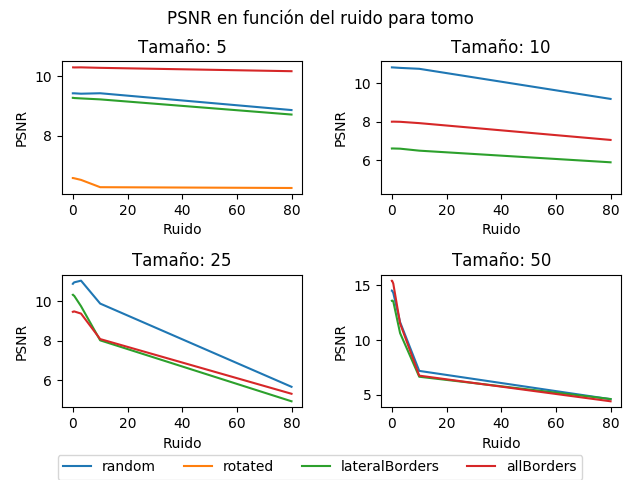
\includegraphics[width=\textwidth]{../graficos/noise/tomo/noise_graph.png}
    \caption{PSNR con respecto a la cantidad de ruido para distintos tamaños de discretización de tomo.png}
    \label{fig:exp-noise-tomo}
\end{figure}

En la figura \ref{fig:exp-noise-tomo}, podemos ver que el ruido afecta más cuanto mayor tamaño de discretización usamos.
% TODO: why?
En los tamaños 5 y 10 de \textit{tomo}, el PSNR parece prácticamente no verse modificado por este.
Sin embargo, con discretizaciones de mayor tamaño,
vemos que el ruido tiene un mayor efecto en las métricas,
principalmente a partir del 10\% de ruido.

También podemos ver que la generación aleatoria de rayos es la mejor con los tamaños del medio (10 y 25),
aunque pasando a la discretización de 50 esta ventaja desaparece.
El método de rayos rotados solo pudo usarse para $n=5$ ya que nuestro modelo de rayos
no nos permite tener la cantidad necesaria para poder probar con mayores \verb|n|
en una imagen con tan poco tamaño original (tomo.png solo mide 100x100 px).

Otra cosa destacable es que recién a partir de la discretización de 50 se puede ver una mejora
en el PSNR, llegando a valores mayores a 15 para ruidos bajos.

\begin{figure}[H]
    \centering
    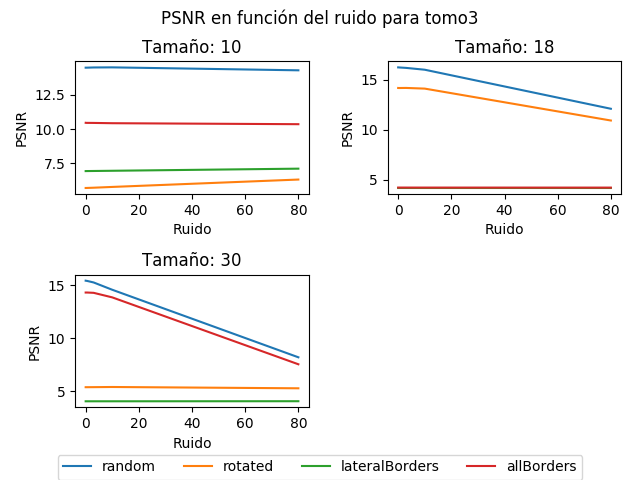
\includegraphics[width=\textwidth]{../graficos/noise/tomo3/noise_graph.png}
    \caption{PSNR con respecto a la cantidad de ruido para distintos tamaños de discretización de tomo3.png}
    \label{fig:exp-noise-tomo3}
\end{figure}

En la figura \ref{fig:exp-noise-tomo3} vemos que el método random es el mejor en todos. Cuando el tamaño es 10 no podemos decir mucho del ruido. Pero luego, para los demás tamaños, vemos que el \verb|PSNR| disminuye a medida que aumentamos el ruido. También podemos observar que a media que aumentamos el tamaño de \verb|n|, los valores de \verb|PSNR| van siendo más similares entre los distintos métodos de rayos. En líneas generales, los resultados son parecidos la figura \ref{fig:exp-noise-tomo}. 

Experimentamos con la tomografía 2 de la figura \ref{fig:tomos} y los resultados dieron también similares a las figuras \ref{fig:exp-noise-tomo} y \ref{fig:exp-noise-tomo3}. No lo incluimos para no repetirnos.


Por lo tanto, podemos concluir que el tamaño de la imagen original no varía en como afecta el ruido al \verb|PSNR|.

A continuación, vemos visualmente cómo se ve la reconstrucción:

\begin{figure}[H]
	\centering
    \begin{subfigure}[t]{0.3\textwidth}
        \centering
        
\includegraphics[height=1.0in]{img/noise/1.png}
        \caption{Tomografía size 10}
    \end{subfigure}
    ~ 
    \begin{subfigure}[t]{0.3\textwidth}
        \centering
        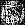
\includegraphics[height=1.0in]{img/noise/2.png}
        \caption{Tomografía size 25}
	\label{tomo:2}
    \end{subfigure}
    ~ 
    \begin{subfigure}[t]{0.3\textwidth}
        \centering
        
\includegraphics[height=1.0in]{img/noise/3.png}
        \caption{Tomografía size 50}
    \end{subfigure}
    \caption{Tomografías reconstruidas del tomo.png con el método random con ruido 0.1}
	\label{fig:resultados-noise1}
\end{figure}

\begin{figure}[H]
	\centering
    \begin{subfigure}[t]{0.3\textwidth}
        \centering
        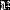
\includegraphics[height=1.0in]{img/noise/4.png}
        \caption{Tomografía size 10}
    \end{subfigure}
    ~ 
    \begin{subfigure}[t]{0.3\textwidth}
        \centering
        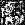
\includegraphics[height=1.0in]{img/noise/5.png}
        \caption{Tomografía size 25}
	\label{tomo:2}
    \end{subfigure}
    ~ 
    \begin{subfigure}[t]{0.3\textwidth}
        \centering
        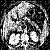
\includegraphics[height=1.0in]{img/noise/6.png}
        \caption{Tomografía size 50}
    \end{subfigure}
    \caption{Tomografías reconstruidas del tomo.png con el método allBorders con ruido 0.1}
	\label{fig:resultados-noise2}
\end{figure}

Se puede ver visualmente que el método random hizo mejor trabajo en reconstruir la imagen.
Esto puede darse ya que nuestra elección arbitraria de rayos haga que se tenga mucha información
de ciertos lugares, y menos de otros, cosa que no sucede al \textit{randomizar} los rayos.


\subsection{Experimentación sobre cantidad de rayos y discretización}
\label{sec:exp-rays}
Además, creemos importante ver cómo la relación rayos/pixeles varía la calidad de los resultados.
A nivel computacional, esto es relevante dado que a mayor cantidad de rayos, mayor tiempo de cómputo,
pero además, si se piensa en el caso de uso de un tomógrafo real,
emitir más rayos implica mayor radiación y peligro para el paciente.

Nuestra hipótesis es que la calidad de las reconstrucciones aumentará con la cantidad de rayos,
hasta un punto en el que se amesetará y dejará de crecer, por las limitaciones del método utilizado.

\begin{figure}[H]
    \centering
    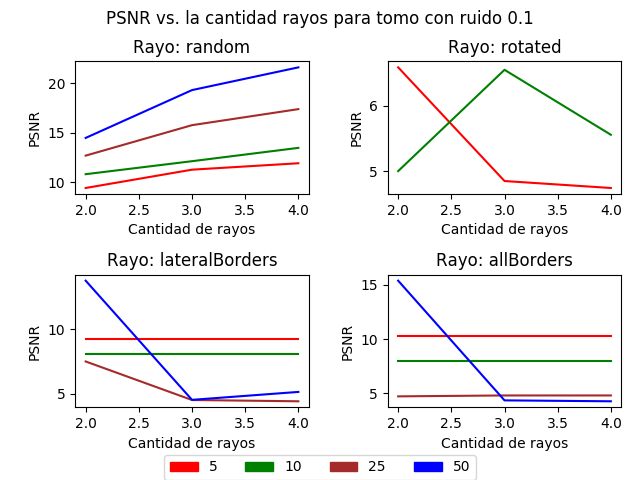
\includegraphics[width=\textwidth]{../graficos/ray_params/tomo/noise_graph_0.png}
    \caption{PSNR con respecto a la relación cantidad de rayos/cantidad de pixeles para distintos tamaños de discretización de tomo.png}
    \label{fig:exp-rayN-tomo}
\end{figure}

Como se puede ver en la figura \ref{fig:exp-rayN-tomo} para el método random estamos en lo cierto. A medida que aumentamos los rayos el \verb|PSNR aumenta|. Lo que no podemos observar es que este valor baje como esperábamos a partir de cierta cantidad de rayos. 

Luego para el resto de los métodos el \verb|PSNR| varia de maneras distintas y es bastante menor que en el random. 

La rotación de rayos podemos ver que no tiene tan buenos resultados comparándola con los otros métodos.
Además, solo lo pudimos correr para un $n=10$ y $n=5$ ya que nuestro modelo de rayos no nos permite tener la cantidad necesaria para poder probar con mayores \verb|n|.

En los últimos dos métodos restantes se observa que agregar más rayos no varia en la imagen final, salvo con $n = 50$. Esto puede pasar gracias a que siempre los rayos están cubriendo gran parte de la imagen necesaria para poder reconstruirla, ya que no son random y están ubicados de forma arbitraria. 

Si se aumenta el n, estamos dejando más celdas en la imagen libres donde puede pasar rayos.
Esto puede justificar por qué con $n = 50$ da mejor \verb|PSNR| en los métodos \verb|allBorders| y \verb|lateralBorders|.
Además puede estar pasando que a medida que se agregan más rayos en lugares fijos a la imagen,
esta se empieze a describir de mala manera y pierda \verb|PSNR|.
Se puede ver que valor de \verb|PSNR| final con $n = 50$ es parecido al del método de rotar.

También vemos el grafico del \verb|tomo3.png| que es un poco distinto al \verb|tomo.png|:

\begin{figure}[H]
    \centering
    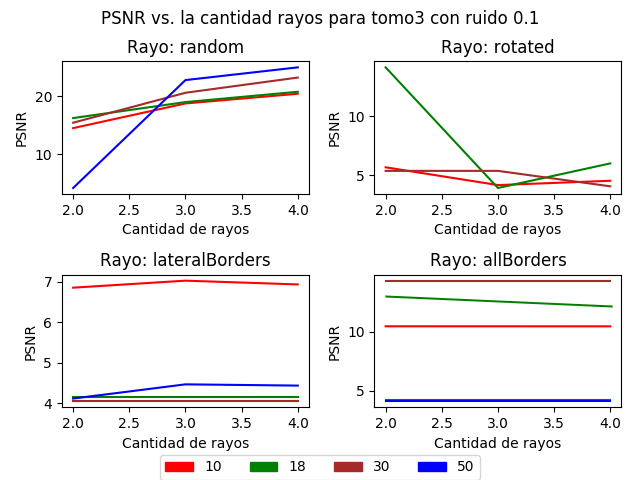
\includegraphics[width=\textwidth]{../graficos/ray_params/tomo3/noise_graph_0.png}
    \caption{PSNR con respecto a la relación cantidad de rayos/cantidad de pixeles para distintos tamaños de discretización de tomo3.png}
    \label{fig:exp-rayN-tomo3}
\end{figure}

En la figura \ref{fig:exp-rayN-tomo3} se puede observar lo mismo en el método random que en la figura     \ref{fig:exp-rayN-tomo}. A medida que aumentamos los rayos el \verb|PSNR| aumenta. Lo que no podemos observar es que este valor baje como esperábamos a partir de cierta cantidad de rayos. También podemos ver en los últimos 2 métodos que agregar más rayos no varía en la imagen final como vimos en la mayoría de los $n$ como en la experimentación anterior. Lo que se puede ver diferente es el método de rotar para $n = 18$, el \verb|PSNR| es más alto que el del método \verb|lateral borders| y parecido al del método \verb|all borders|. Esto parece indicar que la imagen es descripta de mejor manera por los rayos giratorios que tienen forma parecida a los rayos que genera  \verb|all borders|.

Veamos ahora visualmente cómo se reconstruyó una imagen variando la cantidad de rayos:

\begin{figure}[H]
	\centering
    \begin{subfigure}[t]{0.3\textwidth}
        \centering
        
\includegraphics[height=1.0in]{img/ray_n/1.png}
        \caption{Tomografía 150\% del size de rayos}
    \end{subfigure}
    ~ 
    \begin{subfigure}[t]{0.3\textwidth}
        \centering
        
\includegraphics[height=1.0in]{img/ray_n/2.png}
        \caption{Tomografía 200\% del size de rayos}
	\label{tomo:2}
    \end{subfigure}
    ~ 
    \begin{subfigure}[t]{0.3\textwidth}
        \centering
        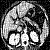
\includegraphics[height=1.0in]{img/ray_n/3.png}
        \caption{Tomografía 300\% del size de rayos}
    \end{subfigure}
    \\
    \begin{subfigure}[t]{0.3\textwidth}
        \centering
        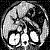
\includegraphics[height=1.0in]{img/ray_n/4.png}
        \caption{Tomografía 400 \% del size de  rayos}
    \end{subfigure}
    ~ 
    \begin{subfigure}[t]{0.3\textwidth}
        \centering
        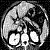
\includegraphics[height=1.0in]{img/ray_n/5.png}
        \caption{Tomografía 500 \% del size de rayos}
    \end{subfigure}
    \caption{Tomografías reconstruidas del tomo.png con el método random con ruido 0.1 de tamaño 50 variando la cantida de rayos}
	\label{fig:resultados-noise1}
\end{figure}

Se puede observar mucha diferencia reconstruyendo entre el 150\% del size de la imagen y entre el 200\% de cantidad de rayos. Luego se ve que la imagen va mejorando a medida que se aumenta la cantidad de rayos pero de manera menos drástica.

% Gráficos de calidad
% Gráficos de tiempo
% Relacion calidad/tiempo?

\subsection{Experimentación sobre cantidad de valores singulares}
\label{sec:exp-eigenvalues}
Como vimos en la sección \ref{sec:exp-noise}, algunas veces, por inestabilidad numérica
o por las propiedades de los rayos, no se pueden encontrar todos los valores singulares.
Pero, dado que estos son los más cercanos a 0, surge el interés de calcular solo los
valores singulares de mayor valor absoluto, que son los que más información nos proveen.
% Agregar en intro teorica cosas sobre low rank approximation y citarlas aca

Esperamos que las métricas bajen al bajar la cantidad de valores singulares.
Sin embargo, nuestra hipótesis consistirá en que esto solo se dará de forma
muy paulatina al principio (dado que la información descartada es poco relevante),
hasta cierto punto en el que las métricas caerán de forma más drástica,
ya que se estará perdiendo información realmente importante.

\begin{figure}[H]
    \centering
    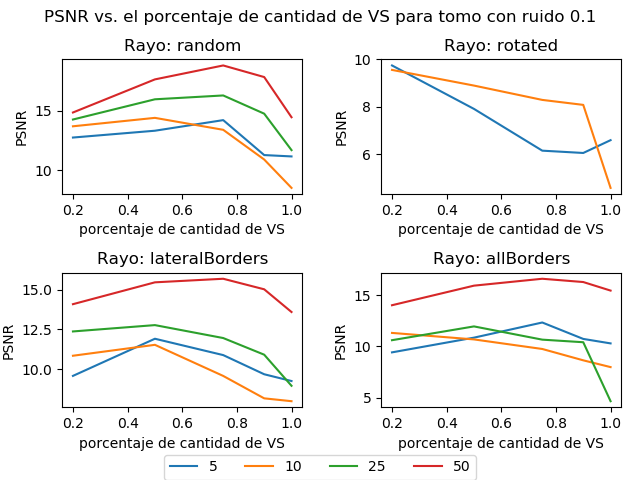
\includegraphics[width=\textwidth]{../graficos/eigens/tomo/noise_graph_2.png}
    \caption{PSNR con respecto al porcentaje de autovalores que calculamos, para distintos tamaños de discretización de tomo.png}
    \label{fig:exp-eigen-tomo}
\end{figure}

Luego de experimentar, notamos que nuestras hipótesis eran erradas.
Como podemos ver en la figura \ref{fig:exp-eigen-tomo}, en general,
dejar de lado algunos autovalores puede incluso hacer que suba el PSNR.
Tanto en el caso de los rayos random, como lateralBorders y allBorders,
suelen alcanzar máximo PSNR al utilizar solo el 75\% de los valores singulares.
Esto puede tener que ver con que los últimos autovalores calculados
arrastran los pequeños errores de muchas iteraciones de deflación,
haciendo que el resultado del Método de la Potencia de resultados que no debería teóricamente.

Sin embargo, hay excepciones.
Con los rayos rotados\footnote{Solo pudimos correr con 2 tamaños de discretización
por las mismas razones que comentamos en los experimentos anteriores},
se puede ver que alcanza máximo calculando muy pocos valores singulares.
Lo mismo sucede en algunos experimentos con otros rayos, con los tamaños de discretización más pequeños.
Intuimos que esto tiene relación con que la cantidad de información a reconstruir es mucho menor,
por lo que los primeros valores singulares son los que realmente da información, mientras que el resto solo agrega ruido.

\subsection{Experimentación sobre tiempo de valores singulares}
Viendo los efectos que tiene la cantidad de autovalores calculados,
nos interesa ver el costo computacional que tiene.
Como vimos en la sección \ref{sec:desarrollo-svd},
calcular cada autovalor tiene un costo de $O(n^2 * 100)$,
dado que hacemos 100 iteraciones con el Método de la Potencia.
Por esto, nuestra hipótesis es que el tiempo aumenta en función de la cantidad de valores singulares a calcular,
en forma cuadrática.

Para comprobarlo, corremos 20 veces nuestro programa con distintos tamaños de discretización
sobre la imagen tomo.png, y tomamos el promedio del tiempo entre el principio y el final del cálculo de CML.
\begin{figure}[H]
    \centering
    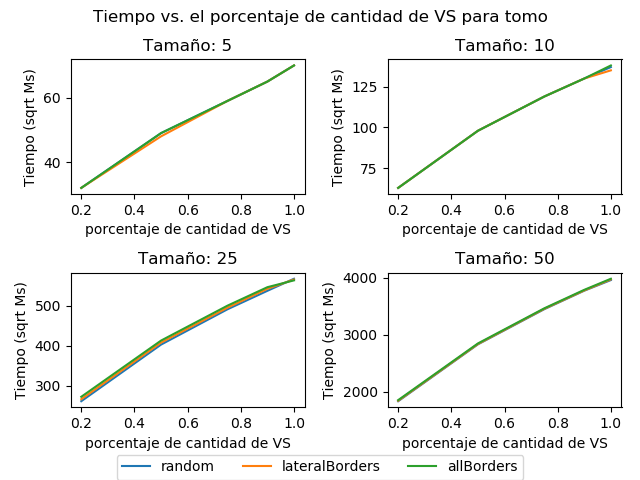
\includegraphics[width=\textwidth]{../graficos/eigens-time/tomo/noise_graph.png}
    \caption{Tiempo de cálculo de CML en función del porcentaje de valores singulares a calcular para tomo.png 
    (escala con raíz cuadrada en el eje vertical)}
    \label{fig:exp-eigenvalues-time}
\end{figure}

Como se puede ver en la figura \ref{fig:exp-eigenvalues-time},
a medida que aumentan la cantidad de valores singulares que deseamos calcular,
también aumenta el tiempo de cómputo para conseguirlo.
Notar que la escala tiene raíz cuadrada en el eje vertical.
Viendo que queda una función prácticamente lineal,
comprobamos que el crecimiento es cuadrático.
Esto comprueba lo que vimos teóricamente.

Con estos resultados, concluimos que es mejor acotar la cantidad de valores singulares a tomar,
ya que permite mejorar las reconstrucciones ahorrando una gran cantidad de tiempo.


\subsection{Experimentación sobre el tamaño de la imagen de salida}
Dados muchos de los resultados anteriores, se nos hace muy interesante enfatizar lo que sucede con la calidad de los resultados
en variación del tamaño de la imagen de salida. Nos interesa saber si efectivamente tamaños más grandes dan como resultado
\verb|PSNR| mayor, y si en algun punto este crecimiento se estanca y resulta innecesario el cálculo de tamaños muy grandes.
Nuestra hipótesis es que a medida que el tamaño aumente, así seguirá el \verb|PSNR|.

\begin{figure}[H]
    \centering
    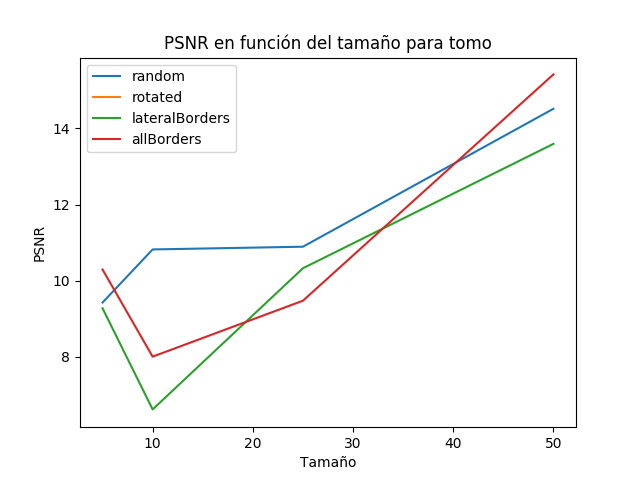
\includegraphics[width=\textwidth]{../graficos/size/tomo/noise_graph.png}
    \caption{PSNR en función del tamaño de la imagen de salida para tomo.png}
    \label{fig:exp-size-1}
\end{figure}

Se puede ver en la figura \ref{fig:exp-size-1} como al aumentar el tamaño de la imagen, también hace crecer el \verb|PSNR|.
% La explicación más directa para este resultado, también es la intuitiva: a más resolución, mejor calidad.
% Sin embargo,  con una explicación más profunda podemos decir que al tener mayor tamaño,
% también tenemos más pixeles de donde sacar información, y estos nos resultan como ecuaciones para nuestras incognitas.
% Por lo que tiene sentido que mayor tamaño den mejores resultados.
Creemos que esto se debe a que al usar discretizaciones muy pequeñas,
se hace que un pixel de la reconstrucción utilice información
de pixeles muy variados de la imagen original,
haciendo que no se parezca en nada a esta.

Algo interesante para destacar, es que si miramos en la figura \ref{fig:exp-eigenvalues-time} podemos ver que mayores tamaños también resultan en
mayor tiempo de cómputo\footnote{En nuestra experiencia con imágenes grandes (90x90), tardan mucho, incluso más de 12hs}. 
Nos encontramos entonces con un \textit{trade-off} entre tiempo y calidad.
